\subsection{GPS-3303}

\begin{figure}[h]
	\centering
	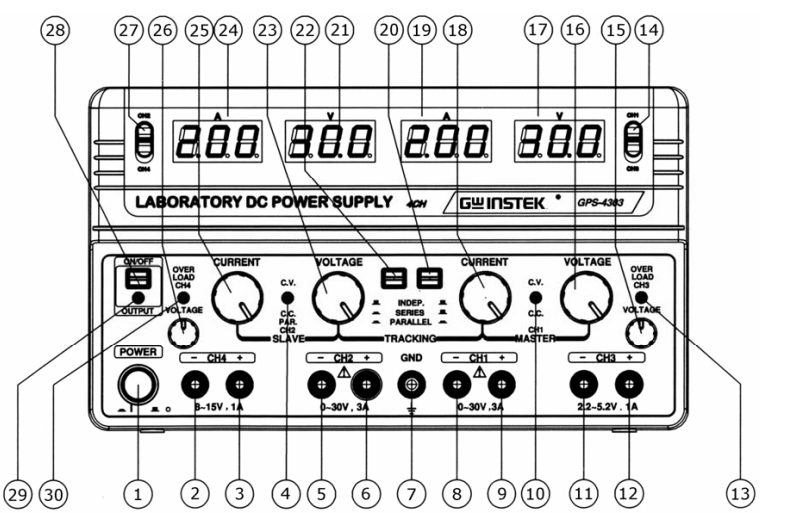
\includegraphics[width=0.7\linewidth]{../Figure/description}
%	\caption{}
	\label{fig:description}
\end{figure}

\begin{enumerate}
	\item
	כפתור הפעלה.
	\addtocounter{enumi}{2}
	\item
	\te{CH2,SLAVE}
	מנורת סימון : \\
	ירוק  = מתח קבוע.\\
	אדום = זרם קבוע.
	\item
	\te{CH2,SLAVE}
	- מחבר יציאה.
	\item
	\te{CH2,SLAVE}
	 + מחבר יציאה.
	 \item
	 \te{GND}
	 מחבר יציאת אדמה.
	 \item
	 \te{CH1,MASTER}
	 - מחבר יציאה.
	 \item
	 \te{CH1,MASTER}
	 + מחבר יציאה.
	 \item
	\te{CH1,MASTER}
מנורת סימון : \\
ירוק  = מתח קבוע.\\
אדום = זרם קבוע.	
	\item
	\te{CH3,CONST:$ \SI{5}{\volt} , \SI{3}{\ampere} $}
	- מחבר יציאה.
		\item
	\te{CH3,CONST:$ \SI{5}{\volt} , \SI{3}{\ampere} $}
	+ מחבר יציאה.
	\item
	\te{CH3,CONST:$ \SI{5}{\volt} , \SI{3}{\ampere} $}
	מנורת סימון שדולק.
	\addtocounter{enumi}{2}
	\item
	
	בורר של \te{CH1,MASTER} מתח.
	\item
	צג מתח,זרם של \te{CH1,MASTER}
	\item
	בורר של \te{CH1,MASTER} זרם.
	\addtocounter{enumi}{1}
	\item
	.22 שליטה של שלושה מצבים :\\
	מצב עצמי(שני הכפתורים משוחררים). \\
	מצב טורי(רק כפתור שמאלי לחץ). \\
	מצב מקבילי(שני הכפתורים לחוצים). 
	
	\item 
	צג מתח,זרם \te{CH2,SLAVE}.
	\addtocounter{enumi}{1}
	\item
		בורר של \te{CH2,SLAVE} מתח.
	\addtocounter{enumi}{1}
	\item
		בורר של \te{CH2,SLAVE} זרם.
	
	\begin{hebrew}
	 	לפירוט נוסף אפשר לפנות ל:
	 	\href{https://www.manualslib.com/manual/811590/Gw-Instek-Gps-2303.html?page=9#manual}{\te{User Manual}}
	\end{hebrew}
	 
	 
\end{enumerate}